\documentclass[a4paper,openright,12pt]{report}
\usepackage[spanish]{babel} % espanol
\usepackage[latin1]{inputenc} % acentos sin codigo
\usepackage{graphicx} % graficos
\usepackage{hyperref}
\usepackage[utf8]{inputenc}
\begin{document}

\begin{titlepage}
%CARATULA
\begin{center}
\vspace*{-1in}
\begin{figure}[htb]
\begin{center}

\includegraphics[width=4cm]{./images/upt}
\end{center}
\end{figure}

UNIVERSIDAD PRIVADA DE TACNA\\
\vspace*{0.15in}
FACULTAD DE INGENIERIA\\
Escuela Profesional de Ingeniería de Sistemas\\
\vspace*{0.6in}
\begin{large}
TEMA : \\
\end{large}
\vspace*{0.2in}
\begin{Large}
\textbf{Tecnologias WAN} \\
\end{Large}
\vspace*{0.3in}
\begin{large}
DOCENTE: PATRICK CUADROS QUIROGA\\
\end{large}
\vspace*{0.3in}
\rule{80mm}{0.1mm}\\
\vspace*{0.1in}
\begin{large}
PRESENTADO POR: \\
Sergio Alexis Ticona Arcaya\\
\end{large}
\vspace*{2in}
\begin{large}
2017\\
\end{large}
\end{center}
%INDICE
\tableofcontents
\begin{large}
\chapter{Introduccion}
\begin{flushleft}
Una red de área amplia, o WAN, (Wide Area Network en inglés), es una red de computadoras que une varias redes locales, aunque sus miembros no estén todos en una misma ubicación física. Muchas WAN son construidas por organizaciones o empresas para su uso privado, otras son instaladas por los proveedores de internet (ISP) para proveer conexión a sus clientes.

Hoy en día, internet brinda conexiones de alta velocidad, de manera que un alto porcentaje de las redes WAN se basan en ese medio, reduciendo la necesidad de redes privadas WAN, mientras que las redes privadas virtuales que utilizan cifrado y otras técnicas para generar una red dedicada sobre comunicaciones en internet, aumentan continuamente..\\
\end{flushleft}


\chapter{Tipos de tecnologías}\label{cap.nudo}
\begin{flushleft}
El modo de transferencia asíncrona (asynchronous transfer mode, ATM) es una tecnología de telecomunicación desarrollada para hacer frente a la gran demanda de capacidad de transmisión para servicios y aplicaciones.

ATM es una tecnología de red que, a diferencia de Ethernet, red en anillo y FDDI, permite la transferencia simultánea de datos y voz a través de la misma línea.

El ATM fue desarrollado para satisfacer las necesidades de la B-ISDN (Broadband Integrated Services Digital Network), tal como fueron definidos en los finales de 1980, y diseñado para unificar las telecomunicaciones y las redes computacionales. Fue diseñado para una red que deba soportar un alto tráfico de datos (ej. Transferencia de archivos), y contenidos como audio y video con poca latencia.
.
\\

\vspace*{0.6in}

\begin{center}
\end{center}
\end{flushleft}

\chapter{Fotos}\label{cap.desenlace}
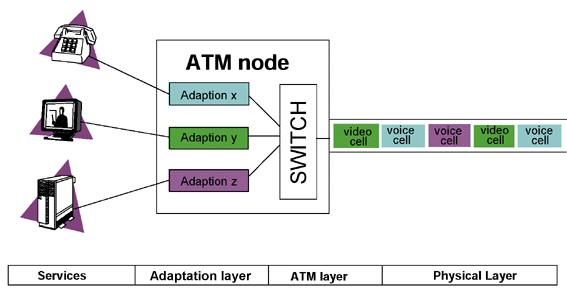
\includegraphics[width=4cm]{./images/1}
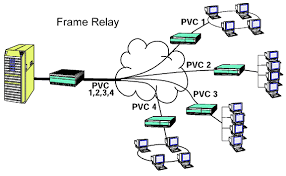
\includegraphics[width=7cm]{./images/2}
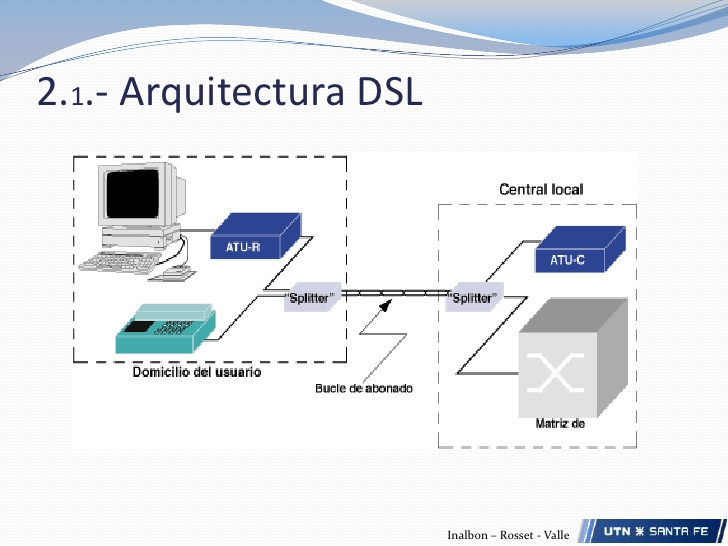
\includegraphics[width=3.5cm]{./images/3}
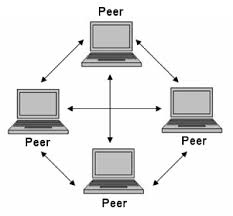
\includegraphics[width=4cm]{./images/4}


\end{large}
%FIN INDICE

\end{titlepage}

\end{document}
